\documentclass[tikz]{standalone}
\usepackage{tkz-graph}
\usepackage{amsmath,amssymb}
\usetikzlibrary{calc}
\usetikzlibrary{positioning}

\begin{document}

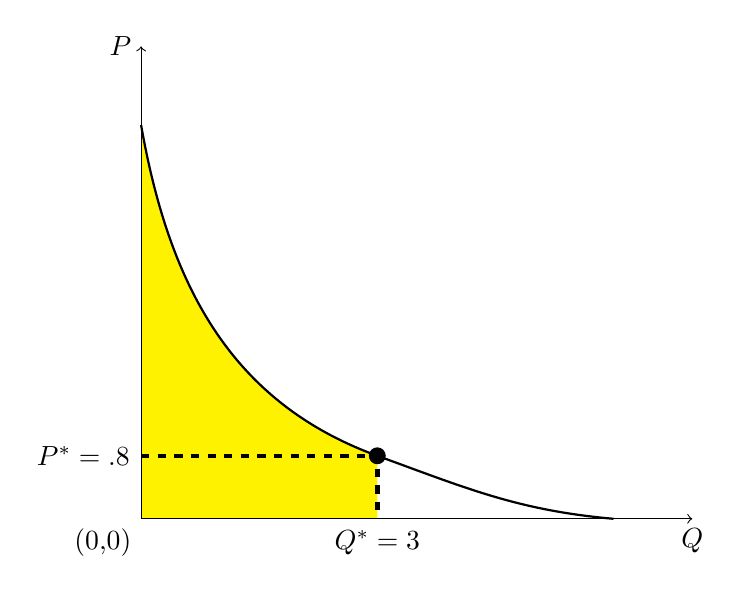
\begin{tikzpicture}
	\path [fill=yellow] (0,0) -- (0,5) to [out=-80, in=160] (3,.8) -- (3,0) -- (0,0);
	\draw [<->] (0,6) node [left] {$P$} -- (0,0) node [below left] {(0,0)} -- (7,0) node [below] {$Q$};
	\draw [ultra thick, dashed] (0,.8) node [left] {$P^*=.8$} -- (3,.8) -- (3,0) node [below] {$Q^*=3$};
	\draw [fill] (3,.8) circle [radius=.1];
	\draw [thick] (0,5) to [out=-80, in=160] (3,.8) to [out=-20, in=175] (6,0);
\end{tikzpicture}

\end{document}




































































































































































































